\documentclass[a4paper,10pt]{article}
\usepackage[utf8]{inputenc}
\usepackage[linguistics]{forest}
\usepackage[round,sort,comma,authoryear]{natbib}

\newcommand{\mli}[1]{\mathit{#1}}

\begin{document}

\begingroup% Robert Frost, T&H p 149
\centering
\vfill
\Huge{Noam Chomsky's}\\[0.5\baselineskip]
\Huge {UNIVERSAL GRAMMAR}\\
\Huge{\&}\\
\Huge{The Current State of The Theory}\\[\baselineskip]
\Large {Samuel Pearce}\par
\large{\scshape 2021}\par
\vfill\null
\endgroup

\begin{abstract}
    Noam Chomsky's Theory of Universal Grammar has been the defining
    theory behind linguistics for the past several decades. Many
    linguists have based their career around how they stand in relation
    to it, and no matter one's stance on the matter, it is impossible
    to refute the Theory's monumental impact on the field as a whole.
    This paper aims to outline --- very briefly --- what the theory
    entails, how it has evolved since it was first proposed in the
    1960s, and what the most current consensus on the matter is.
\end{abstract}

\pagebreak


\tableofcontents
\pagebreak


\section{Universal Grammar}
To begin with, what is universal grammar exactly, and what does it entail? Well, contrary to what
I originally thought, it is not a defined linguistic grammar that applies to all human languages.
The theory of universal grammar mainly consists of the hypothesis that language is an innate human
faculty that is defined --- at least, to some extent --- by our biology and genetics. One of the
well-known arguments Chomsky presents is that young children can understand grammatical concepts
about the language they speak without having been taught it directly.\citep[p.~26]{ChUGAI}

At its base, UG-theory suggests there is some kind of ``computation system'' that converts the
external signals (sounds, symbols, sign-language, etc.) into internal ideas. \citep[p.~5]{ChUGAI}
Most of what Chomsky worked on after the theory was put into place, was creating a formal system
to analyse syntax of varying languages to compare which elements could be universal. The ideas
and structures used to analyse language and form ideas about how such an internal system might
be structure has been discussed and evolved over the past nearly half century:
\begin{quote}
	``The UG Theory claims to be a scientific theory based on solid evidence about language.
	As such, it is always progressing towards better explanations for language knowledge....''
	
	\citep[p.~27]{ChUGAI}
\end{quote}

The theory split into two main branches, each focusing on one end of the computational system;
they were the ``E-Language'' and ``I-Language'' branches. E-Language is primarily concerned with
the actual physical manifestation of language by gathering large samples and analysing them. The
I-Linguists focus on mapping out how these ideas are stored in the brain, whith the details of
how they are expressed mostly irrelevant. To summarise: E-Language ``is concerned with what people
have done'', while I-Language ``is concerned with what they could do'' \citep[p.~14]{ChUGAI}

One of the first things one would think to analyse when speaking about a ``universal'' grammar
are so-called linguistic universals; features that have the same structure throughout all human
languages. Greenbergian universals, linguistic features like syntax structure or movement rules
that appear in all natural languages \citep{Greenberg473}, differ from Chomskyan universals in that
Chomskyan universals needn't manifest in every language; ``No language violates a universal principle
(the language simply may not use the principle in a particular context)'' \citep[p.~23]{ChUGAI}


\section{Generative Grammar}
A generative grammar is a description of a language that uses a very explicit syntactic syntax.
Chomsky himself defined it thusly:

\begin{quote}
	``When we speak of the linguist's grammar as a `generative grammar' we mean only that it is
	sufficiently explicit to determine how sentences of the language are in fact characterised
	by the grammar''
	
	\citet[p.~220]{Chomsky80}
\end{quote}

It is based on the idea of building up sentence syntax the same way one can with
a mathematical grammar, like a programming language, possible syntax trees are written as recursive
rewrite rules such as:

\[        S \rightarrow \mli{NP} \; \mli{VP} \]
\[ \mli{VP} \rightarrow V        \; \mli{NP} \]
\[ \mli{NP} \rightarrow Det      \; N        \]

In the above example a sentence (S) is defined as a noun-phrase (NP) plus a verb-phrase (VP),
a verb-phrase consists of a verb (V) and a noun-phrase, and a noun-phrase is a determiner (Det) plus
a noun (N). With these rules you can construct some of the many possible grammatically valid sentences
for English. \citep[p.~32]{ChUGAI}

Though this was just the beginning of a new way of analysing the syntactic structures of sentences
which lead to many further developments.


\section{Government/Binding Model}
In the new government/binding model, the simple building blocks of language which were still being
defined were stuck together modularly to create a model of how the computational system could be
structured. At its base, the structure has two layers: the D-structure (deep structure) and the
S-structure (surface structure). The D-structure reflects the base grammatical structure of the
sentence, influenced by the lexicon and phrase structure rules explained above, while the S-structure
is what is actually said after being adjusted by movement rules. \citep[p.~61]{ChUGAI}
For example, in the following sentence, the ``whom'' would be the object of the sentence --- coming
after the verb as usual --- in the D-Structure, but because it's a question, the object is moved
to the front of the sentence:

\begin{center}
	* You did see whom. $\rightarrow$ Whom did you see?
\end{center}

This was the basis of the GB theory which would continue to be developed with new additions to
help handle all cases seen in human languages that didn't already meet the basic model. One of
the first iterations of the model, as described above, is illustrated in the following figure
from \citet[p.~62]{ChUGAI}

\begin{center}
	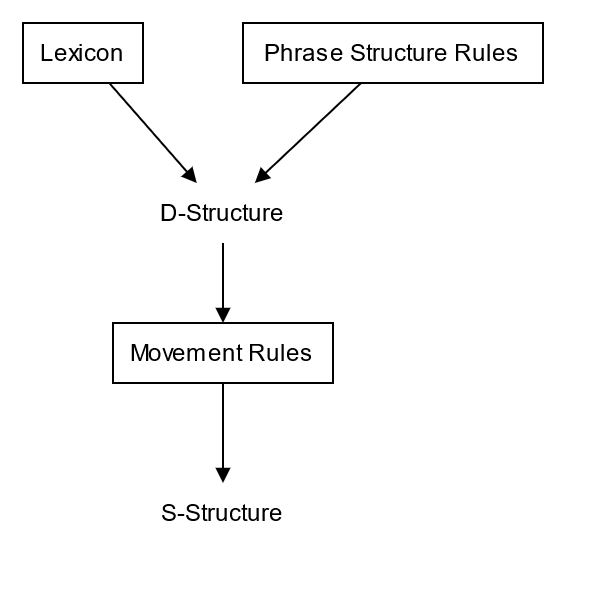
\includegraphics[scale=0.25]{gb-model-init.png}
	\linebreak
	Fig. 1: One of the simplest forms of the GB-Model
\end{center}


\section{X-Bar Theory}
In the earlier example we stated that a verb-phrase was defined as a verb and a noun-phrase, but
some verbs are intransitive and don't take an object. While we could simply define two possible
verb-phrase trees --- one with a object and one without --- this information is based on the word
itself and this causes an unnecessary redundancy. Chomsky's rewrite rules were then expanded upon
with the introduction of X-bar notation to remove this redundancy; a phrase could be defined using
only following rewrite rules:

\[ X'  \rightarrow  \mli{X}   \; (\mli{YP})\footnotemark[1] \]
\[ X'' \rightarrow (\mli{YP})\footnotemark[2] \;  \mli{X'}  \]

\footnotetext[1]{The complement is optional, it is determined by the head}
\footnotetext[2]{The specifier is also optional, but isn't selected by the head}

\begin{center}
	\begin{forest}
	[X$^{\prime\prime}$
		[specifier]
		[X$^{\prime}$
			[X]
			[complement]
		]
	]
	\end{forest}
	\linebreak
	Fig. 2: The X-Bar rules displayed in a tree
\end{center}

Substitute X and Y with any of the four lexical categories in the theory
--- Noun (N), Verb (V), Adjective (A), Preposition (P) --- and you have the structure of that phrase.
This system can represent any phrase possible by recursively adding more elements to the tree.
\citep[p.~66]{ChUGAI}

\begin{center}
\begin{forest}
[S
	[N$^{\prime\prime}$ [he, roof]]
	[V$^{\prime\prime}$
		[V$^{\prime}$
			[V [flew]]
			[P$^{\prime\prime}$
				[P$^{\prime}$
					[P [to]]
					[N$^{\prime\prime}$ [London, roof]]
				]
			]
		]
	]
]
\end{forest}
	\linebreak
	Fig. 3: An example of recursive phrases from \citet[p.~68]{ChUGAI}
\end{center}


\section{Principles \& Parameters Theory}
Principles and Parameters (P\&P Theory) is a continuation of the GB-model which more accurately represents
the more general nature of GB theory.

\begin{quote}
	``These modules of language stand alongside many others ... Determination of of the nature of
	of these and other systems is a common project, not specific to this particular conception
	of the nature of language and its use''
	
	\citet{Chomsky95}
\end{quote}

Principles replaced the idea of fixed grammatical rules with a more generic set of constraints that
apply to all constructions in a language as opposed to very specific ones, as with ordinary rules.
\citep[p.~35]{ChUGAI} An example of a Principle as provided by is the principle
of locality:

\begin{quote}
	``\textbf{Locality:} this principle is a property of linguistic processes which restrics their
	application to a limited part of the sentence. This then forces movements in all languages to be
	local: \emph{they must be short.}
	
	\citet[p.~41]{ChUGAI}
\end{quote}

Parameters are what account for the wide variation we see between languages; if the only thing governing
languages were a set list of principles, they would be far more similar than they are.
\citet[p.~44]{ChUGAI} use the head parameter to illustrate how parameters differ from principles:
The head is the most important word in a phrase; it selects what kind of complements may
be used with it. Depending on the language, this word may come before or after its complement
(or either side such as in French). While it is a principle that a phrase must have a head, where
it goes is decided by the head parameter and differs from language to language.

With P\&P theory and X-bar notation, the GB-model was expanded to include far more modules
over the course of many years of study, leading to the following version of the model:

\begin{center}
	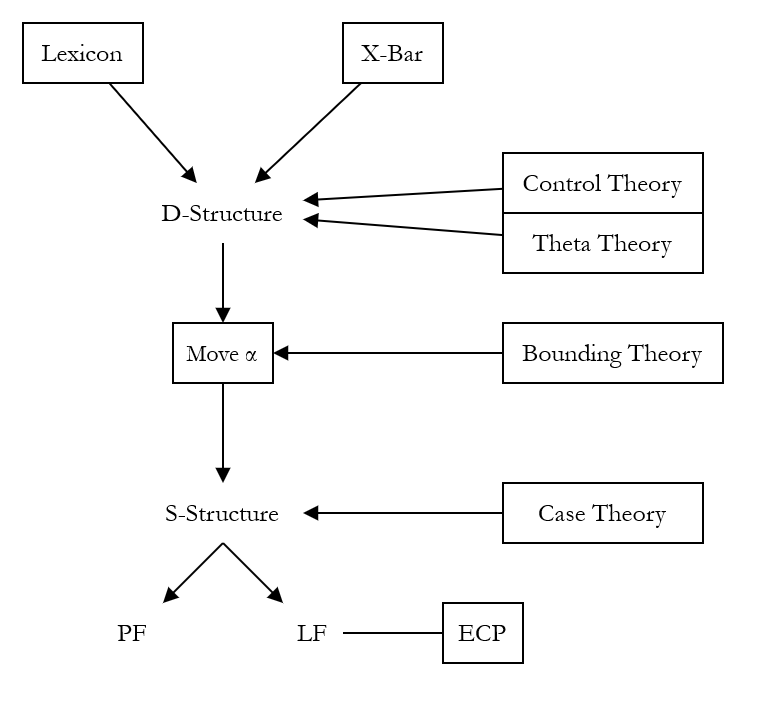
\includegraphics[scale=0.25]{gb-model-end.png}
	\linebreak
	Fig. 4: The structure of the current GB-model \citep[p.~181]{ChUGAI}
\end{center}


\section{Minimalist Program}
The minimalist program is the name for the latest (since 2000) development out of the GB and P\&P
Theories. it espouses any claims at definitivenes by its name; it's a program at the moment, not a
developed theory; it's the approach being taken to explore the most recent and least-well understood
linguistic concepts. \citep[p.~242]{ChUGAI}
So far, the minimalist program has had very little impact on language acquisition research specifically:
``Most L1 researchers seem quite happy to continue using a version of the P\&P model that involves
little of the MP'' \citep[p.~219]{ChUGAI}

The minimalist program had three main phases of its development: in the beginning, it focused on
finding the most foundational principles of the worlds languages and the principles which made up
for the discrepancies between them. After that, the linguists began examining how perfect the interface
between the phonetic form (PF) and the computational system.a large portion of the GB-model was demolished
in order to reconstruct the syntax tailored to the most minimal ideas. \citep[p.~3]{ChUGAI}
After that, The phases model has been the latest production of the minimalist program. One can
read about the phases model from \emph{The Architecture of Language} \citet{Carr05}


\section{Criticism}
Chomsky's theory of Universal Grammar has been the subject of relentless criticism since it first
came about in the 1960s. One of the most common argument that targets the foundation of the concept
as a whole criticises the assumption that psychological theories can be evaluated in the same way
physical ones can; some, such as \citet{Quine60} claimed they are not the same. Chomsky rebutted this
by explaining his view that there is no proof that one cannot distinguish between two psychological
theories. \citep[p.~13]{Cipriani15}

Another point often brought up is that the principles in P\&P theory must limit the scope of
human language, no matter how extensive the parameters alter their representations. Though, this
can be fairly easily dismissed as it is an inherent property of the theory; if you want to make
a list of things which are common to all languages, it must have a fixed boundary to have any
meaningful value. \citep[p.~13]{Cipriani15}

A very strong criticism levied against UG is that it has no limit to how many exceptions it can have
while still being considered correct. In other fields such as mathematics, you would have to abandon
a theory once it exceeded the ideal limit of exceptions, but UG is always correct. The consequence
of this is that UG theory is not falsifiable, and therefore --- according to some --- unscientific.
\citep[p.~14]{Cipriani15}


\section{My Impression}
Personally, I find the last of the example criticism very compelling; as I read through \citet{ChUGAI},
I found myself often lamenting the rapid loss of elegence in any new concept introduced. At the time,
I couldn't put into words the feeling that this \emph{couldn't} be universal; there were far too many
exceptions and specific rules that it seemed to only apply to a handful of very well-known languages
like English, German, Japanese, etc. Likely this is due to the very brief introduction I have been
given, but I still feel it's unproductive to analyse something that, it seems, we will never be able
to prove. I'm very appreciative of the many positive impacts UG's study has had on the entire field of
linguistics and computer-science, I can't help feel it's unscientific to make claims about the extremely
subjective qualia of human language. It makes a fantastic \emph{model} of human languages in, probably,
the most elegant manner, but --- at least for now --- it can only ever be a model.

Another concept troubling me while studying this is that it seems to miss a question that interests
me greatly: are human languages representative of the full extent of human language faculty (assuming
it is a biological faculty)? How can we tell where the border of this in-built faculty is? It's possible
that we could learn more complex languages, or simply completely different languages from what seems
possible given all current knowledge of human language, but this is taken up by other parts of the
brain and could seem indistinguishable from regular language faculty. Does this simply also count as
part of UG, or is this the brain simply adapting to a new language by using it's other logical
faculties?

These questions were prompted by my interest in constructed languages (conlangs) such as
Toki Pona \citep{Lang14} and Ithkuil \citep{Quijada11} which test the extreme limits of our language
faculty. I would be interested to know how these fit into UG theory, if they do at all, because their
ability to test what we can interpret as ``langauge'' seems to suggest to me that while we are probably
equipped to develop, speak and understand language by evolution, it might be far more open-ended than
we previously thought. Personally, I think the negative stigma still attached to conlangs and the
prevailing opinion that they aren't ``real languages'' might be hindering linguistic progress.
I think that, until we can fully accept conlangs as valid and powerful avenues of linguistic exploration,
making any significant progress towards understanding language and human nature as a whole will be
stunted.


\pagebreak
\bibliographystyle{plainnat}
\bibliography{Bibliography}

\end{document}
